\section{Protocols}

\subsection{Master}

The master process is responsible for connecting to the coordinators, sending them configurations, and waiting for their final responses. Since it needs to complete only a linear sequence of steps, it runs in a single thread.

The master process begins by reading a configuration file with a list of IP addresses and ports at which coordinators can be reached. It also reads data about the world size, terrain, and the locations of agents. It then decides which agents will be managed by which coordinators and which coordinators will be \emph{neighbors}, i.e. which coordinators will maintain connections to each other.

It opens a TCP connection with each coordinator and sends the configuration information, then waits for confirmations from all coordinators that the information was received (\texttt{CONFIG\_CONFIRM}). It then waits for a second confirmation that all agents were launched successfully (\texttt{READY}) and the simulation can begin.

\begin{figure*}
    \begin{center}
        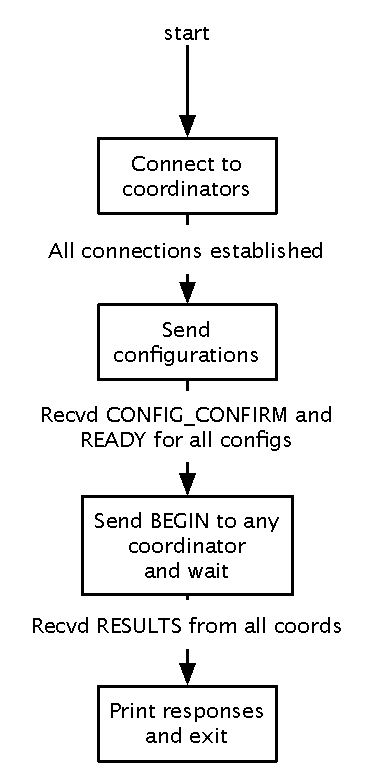
\includegraphics[scale=0.5]{figures/state_master.pdf}
    \end{center}
    \caption{State transition diagram for the master process.}
    \label{master}
\end{figure*}

To start the simulation, the master process sends \texttt{BEGIN} to any coordinator. It then waits for all coordinators to report back to it with information about the end of the simulation (RESULTS). Finally, it prints all relevant results.

A state transition diagram of this process is shown in figure \ref{master}.

\subsection{Coordinator}

The coordinator is the most complex part of the system. At any given time, as many as four threads may be running simultaneously. The full state transition diagram is shown in figure \ref{coord}.

At the high level, the coordinator connects to neighbors and agents, serves requests for information about the state of its agents in the last turn, and processes its own agents by requesting information from its neighbors and from its agents.

\subsubsection{The main thread}

The main thread handles the lifecycle of the coordinator and those of its connections. It begins by listening for a TCP connection from the master process. Once connected, it reads its configuration, which contains IP addresses/ports at which its neighbors are listening for it, which agents it should launch, and where to place them. It sends \texttt{CONFIG\_CONFIRM} back to the master process.

Coordinators are connected to each neighbor by two TCP connections. The coordinator listens on one of these for requests for information from the neighbor. It uses the other to request information of the neighbor. These connections are established using information sent from the master process.

Coordinators are connected to actors by a single TCP connection. To begin the agent communication process, the coordinator launches the agent process and repeatedly tries to open a socket to it until it responds.

The connections to the neighbors and agents are all established at once, asynchronously. When all connections are established, the coordinator sends READY to the master process and launches the \texttt{listenMaster} and \texttt{listenPeers} threads.

It waits for two locks, \texttt{TCOMPLETE1} and \texttt{TCOMPLETE2}, to be released. After these locks are released, the coordinator sends information about the final state of its agents back to the master process and exits, sending exit messages to the agents as well.

\begin{figure*}
    \begin{center}
        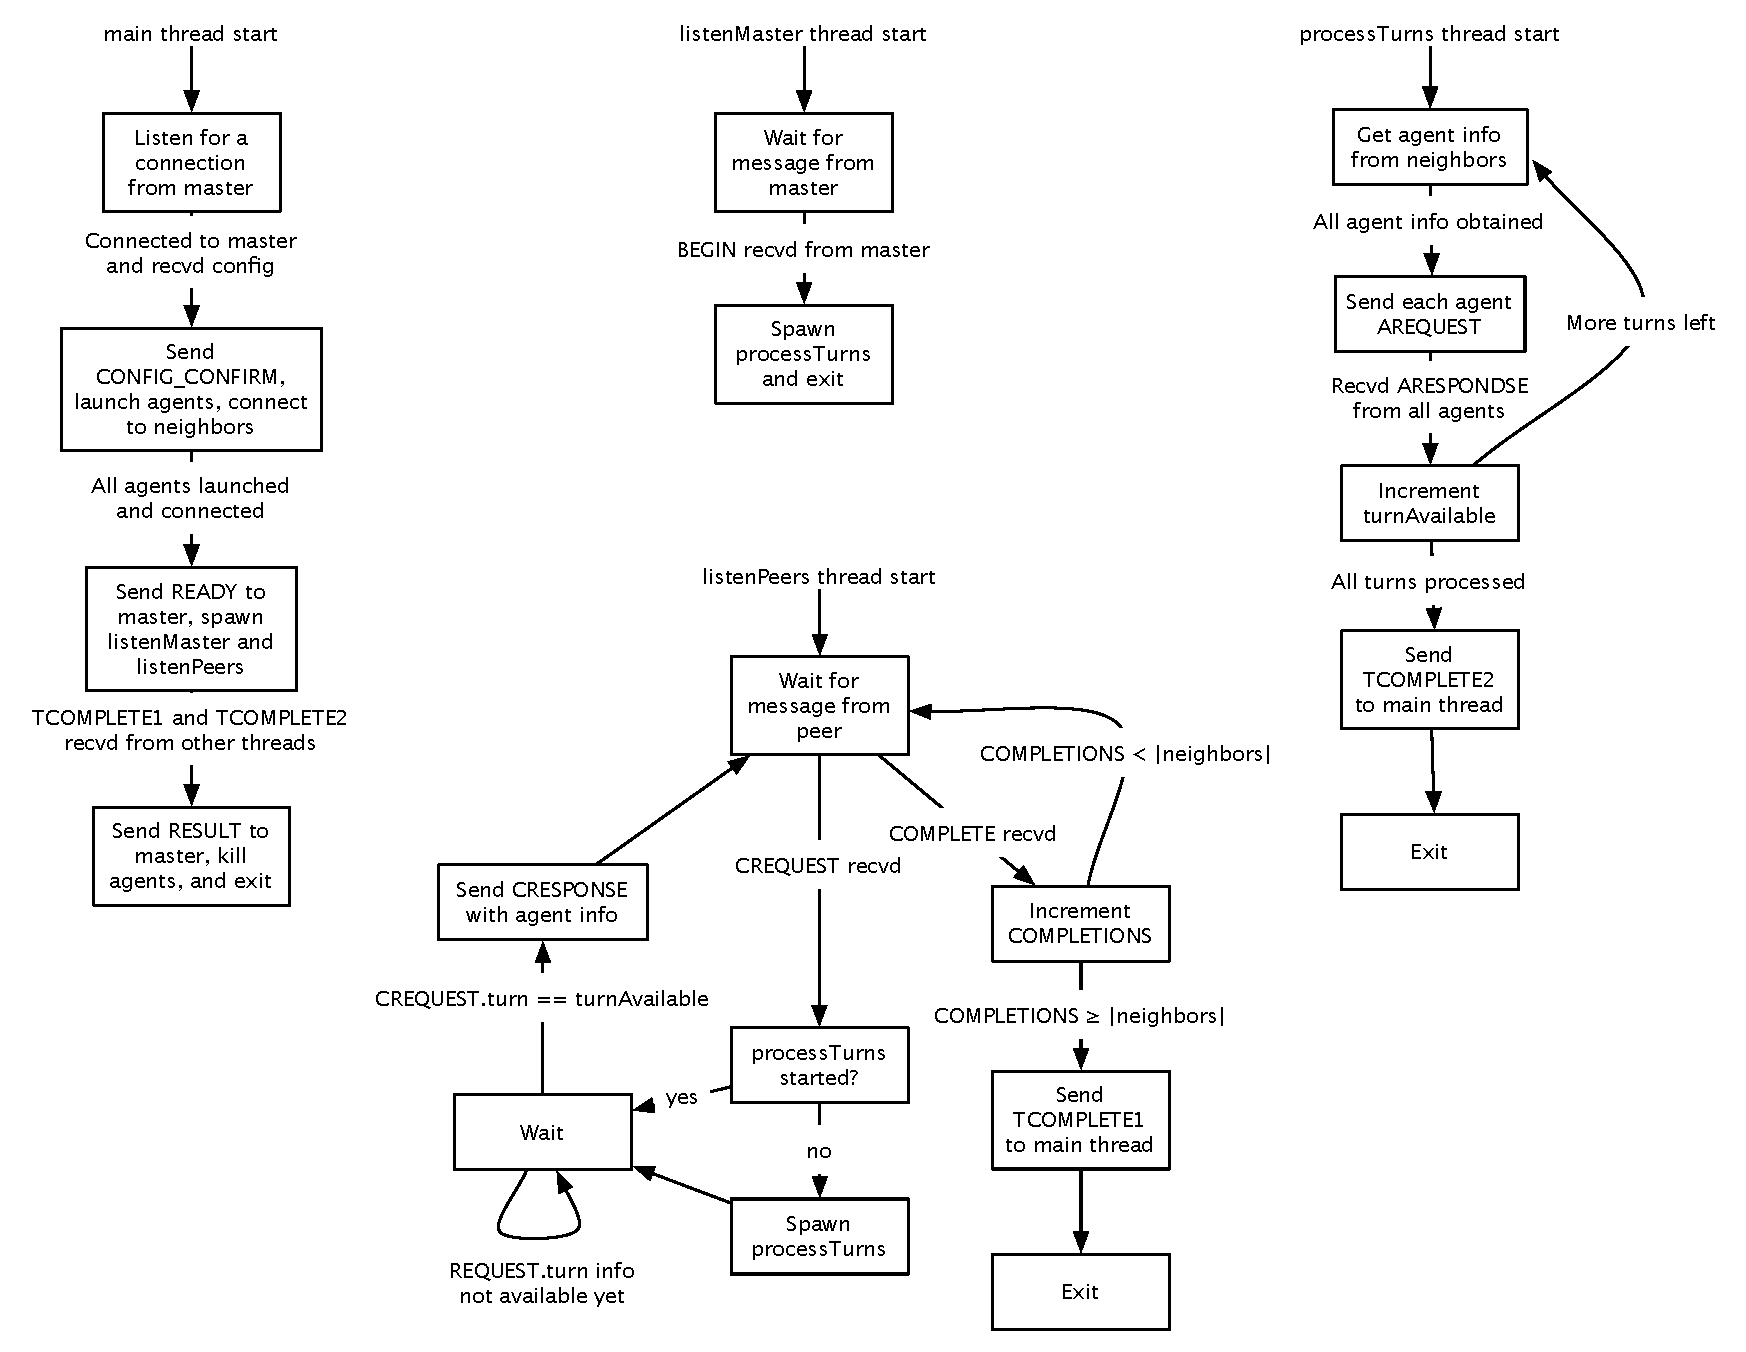
\includegraphics[scale=0.5]{figures/state_coord.pdf}
    \end{center}
    \caption{State transition diagram for the coordinator processes.}
    \label{coord}
\end{figure*}

\subsubsection{The listenMaster thread}

The master process begins the simulation by sending \texttt{BEGIN} to any coordinator. This message is received by the \texttt{listenMaster} thread, whose only job is to spawn the \texttt{processNodes} thread and exit.

\subsubsection{The listenPeers thread}


